\chapter{Algorithme de résolution}





L'algorithme de résolution est implémenté dans la classe \texttt{Ordi(Joueur)} du module \texttt{bn\_joueur.py}, dans la méthode \texttt{Ordi.coup\_suivant(self)}. L'attribut \texttt{Ordi.case\_courante} contient la case qui est entrain d'être jouée.

Il fonctionne en deux temps : dans un premier temps une phase de tir en aveugle et, une fois qu'une case a été touchée, une phase de tir ciblé jusqu'à ce que le bateau soit coulé.

Différents algorithmes de résolution sont implémentés et choisis avec l'attribut \texttt{Ordi.niveau} :
\begin{itemize}
\item \texttt{Ordi.niveau=1} : Uniquement des tirs aléatoires en aveugle et pas de tirs ciblés.
\item \texttt{Ordi.niveau=2} : Tirs aléatoires et phase de tirs ciblés.
\item \texttt{Ordi.niveau=3} : Tirs aléatoires sur les cases noires  et phase de tirs ciblés.
\item \texttt{Ordi.niveau=4} : Détermination de la case optimale par des échantillons et phase de tirs ciblés.
\item \texttt{Ordi.niveau=5} : Détermination de la case optimale par le nombre de bateaux possibles sur chaque case et phase de tirs ciblés.
\item \texttt{Ordi.niveau=6} : Idem niveau 5, mais dès que le nombre de cases vides passe en-dessous de \texttt{Ordi.seuil}, l'algorithme énumère toutes les répartitions de bateaux possibles.
\end{itemize}

Une étude statistique de chacun de ces algorithmes est donnée en annexe \ref{annexe_stats}, page \pageref{annexe_stats} et un exemple de résolution pas à pas (avec le niveau 5) est donné dans l'annexe \ref{annexe_algo_action}, page \pageref{annexe_algo_action}. L'algorithme complet de résolution est donné en annexe \ref{algo_liste}, page \pageref{algo_resolution}.




\section{Phase de tir en aveugle}
Lors de cette phase, l'algorithme va commencer par éliminer les zones dans lesquelles le plus petit bateau restant ne peut pas rentrer, puis choisir une case aléatoire parmi les cases vides. Le choix de cette case va, en grande partie, déterminer les performances de l'algorithme.

\subsection{Tirs aléatoires}

\subsubsection{Méthode naïve}
La méthode la plus naïve est de choisir une case de manière uniforme dans la liste des cases vides avec l'instruction \texttt{random.choice(liste)}.

Cette méthode est celle qui peut être attendue d'un élève (qui peut se contenter de ça pour l'ensemble de son algorithme de résolution) et la seule qui permette de résoudre la grille uniquement en faisant des tirs en aveugle.

\subsubsection{Méthode des cases noires}
Dans la mesure où le plus petit bateau est de taille 2, si on imagine la grille comme un damier, un bateau recouvre obligatoirement une case noire. On peut donc se contenter de viser uniquement parmi ces cases.

Une case $(x,y)$ est une case noire si, et seulement si, $(x+y)\%2==0$.

\subsection{Optimisations}

\subsubsection{Méthode par échantillonnage}
Dans la méthode suivante, on va essayer d'optimiser les tirs en aveugle en estimant la probabilité de chaque case de contenir un bateau.

Pour ce faire, on va créer un échantillon de $n$ répartitions aléatoires de bateaux sur les cases vides restantes et on va compter, sur chacune, le nombre de fois où elle a été occupée ce qui va nous donner une densité de probabilités pour chaque case. Cette partie est gérée par la méthodes \texttt{Grille.case\_max\_echantillons(self, nb\_echantillons)} dont l'algorithme est donné en annexe \ref{algo_liste}, page \pageref{case_max_echantillons}.

%\begin{algo1}
%probas est un dictionnaire indexé sur les cases\\
%Pour chaque case, 0\sto probas[case]\\
%On répète nb\_echantillons fois :\\
%\tab{1}grille\_tmp reçoit une copie temporaire de la grille du suivi\\
%\tab{1}On crée une flotte aléatoire sur grille\_tmp\\
%\tab{1}Pour chaque case vide dans la grille de suivi originale :\\
%\tab{2}Si la case contient un bateau dans grille\_tmp :\\
%\tab{3}probas[case]+1\sto probas[case]\\
%Pour chaque case, probas[case]/nb\_echantillons\sto probas[case]\\
%case\_max est la case qui a la plus grande probabilité pmax\\
%On retourne (case\_max, pmax)\\
%\end{algo1}

Les performances en nombre d'essais sont satisfaisantes, mais le temps de calcul beaucoup trop élevé. 
\begin{comment}
Voici un tableau récapitulatif de quelques essais avec différents paramètres :

\medskip

\begin{center}
\begin{tabular}{|l|c|c|c|c|}
\hline
Taille des échantillons & 100 & 1\,000 & 10\,000 & 100\,000\\
\hline
Nombre de parties & 10\,000 & 10\,000 & 1\,000 & 100\\
\hline
Nombre de coups moyens & 43,68 & 43,30 & 42,72 & 42,63\\
\hline
Temps moyen par partie (en secondes) & 0,38 & 3,6 & 36,2 & 380\\
\hline 
\end{tabular}\\
\vspace*{0.1cm}
\textit{Temps mesurés sur un processeur Intel Core i7 4800-MQ à 2,7 GHz}
\end{center}

\medskip

Au final, le temps de résolution est linéaire en $n$ pour des gains de performances négligeables.\\ Le calcul est effectué dans la méthode \texttt{Grille.case\_max\_echantillons(self, nb\_echantillons, ordre)} du module \texttt{bn\_grille.py}.
\end{comment}
 
\subsubsection{Méthode par énumération de tous les cas}

On peut essayer de déterminer tous les arrangements de bateaux possibles sur la grille à chaque coup, de manière récursive. Cette approche semble optimale mais malheureusement, vu le nombre de configurations, cette approche est inutilisable sur une grille standard. Elle est néanmoins implémentée dans la méthode \texttt{Grille.case\_max\_all(self)}.

\subsubsection{Méthodes par comptage}
Dans cette méthode, on va compter pour chaque case le nombre de bateaux possibles contenant celle-ci et tirer sur celle qui en contient le plus.

La méthode \texttt{Grille.case\_max(self)} renvoie la case optimale, ainsi que le nombre de bateaux qu'elle contient. L'algorithme est donné en annexe \ref{algo_liste}, page \pageref{case_max}.

%\begin{algo1}
%probas est un dictionnaire indexé sur les cases\\
%Pour chaque case, 0\sto probas[case]\\
%On récupère la liste des bateaux possibles sur chaque case\\
%\tab{1} (dans le dictionnaire possibles)\\
%Pour chaque taille de bateau restant :\\
%\tab{1}Pour chaque (case, direction) permettant de démarrer le bateau :\\
%\tab{2}La probabilité de chaque case occupée par le bateau est augmentée de 1\\
%case\_max est la case qui a le plus de possibilités pmax\\
%On retourne (case\_max, pmax)\\
%\end{algo1}

%L'algorithme est très simple : d'abord on crée un dictionnaire \texttt{Grille.probas} indexé par les cases et contenant le nombre de bateaux possibles grâce à \texttt{Grille.possibles}. Ensuite il ne reste plus qu'à renvoyer celle qui en contient le plus.

Bien que locale (on ne regarde pas la répartition de tous les bateaux ensemble sur la grille), cette méthode est très efficace.




\section{Phase de tir ciblé}
Lors de cette phase, on va utiliser une file d'attente dans la liste \texttt{Ordi.queue} qui va contenir la liste des prochaines cases à viser. On va également garder la trace des cases touchées sur ce bateau dans la liste \texttt{Ordi.liste\_touches}, ainsi que sa première case touchée dans \texttt{Ordi.case\_touchee}.
\subsection{Premier tir}
\subsubsection{Création de la liste des cases adjacentes}
Lors du premier tir touché après la phase de tir en aveugle, l'attribut \texttt{Ordi.case\_touchee} reçoit la case courante qui sera également ajoutée à \texttt{Ordi.liste\_touches}. Puis on va remplir la file d'attente avec les cases adjacentes à la case touchée.

L'algorithme va également vérifier si le plus petit bateau ne peut pas rentrer dans une direction. Imaginons, par exemple, que le plus petit bateau restant soit de taille 3 et qu'on vienne de toucher la case $(3,0)$ dans la configuration suivante :

\begin{center}
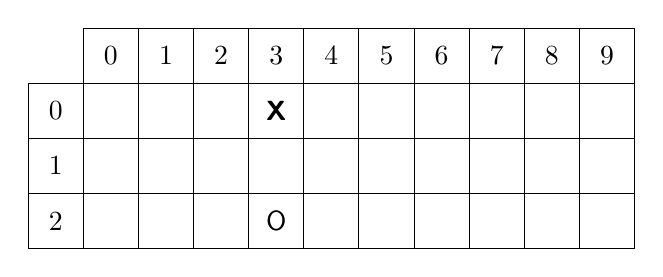
\begin{tikzpicture}[scale=0.7]
\draw (0,1)--(10,1);
\draw (-1,0)--(10,0);
\draw (-1,-1)--(10,-1);
\draw (-1,-2)--(10,-2);
\draw (-1,-3)--(10,-3);
\foreach \x in {0,1,...,10}{
\draw (\x,1)--(\x,-3);
}
\draw (-1,0)--(-1,-3);
\foreach \x in {0,1,...,9}{
\draw (\x+0.5,0.5) node{\x};
}
\draw (-0.5, -0.5) node{$0$};
\draw (-0.5, -1.5) node{$1$};
\draw (-0.5, -2.5) node{$2$};

\draw (3.5, -0.5) node{\textbf{\textsf{X}}};

\draw (3.5, -2.5) node{\textsf{O}};
\end{tikzpicture}\\
\textit{Le bateau de taille 3 ne rentre pas verticalement}
\end{center}
Il ne sert alors à rien de mettre la case $(3,1)$ dans la file d'attente car le plus petit bateau de taille 3 ne peut pas rentrer verticalement en $(3,0)$.

La construction de la liste des cases adjacentes possibles est effectuée par la méthode \texttt{Ordi.add\_adjacentes\_premiere(self)} dont l'algorithme est donné en annexe \ref{algo_liste}, page \pageref{add_adjacentes_premiere}.

\subsubsection{Optimisation de la file d'attente}

Pour l'optimisation de cette phase, on va classer la file d'attente en ordre décroissant de nombre de bateaux possibles avec la méthode \texttt{Ordi.shuffle\_queue(self)}.
 
Cette optimisation est un petit peu délicate. Une fois qu'une case a été touchée, l'algorithme va tester ses 4 (au maximum) cases adjacentes et les ranger en ordre décroissant du nombre de bateaux possibles. C'est le rôle de la méthode \texttt{Grille.case\_max\_touchee(self, case\_touchee)}, dont l'algorithme complet est donné en annexe \ref{algo_liste}, page \pageref{case_max_touchee}. 

\medskip

Notons \texttt{(x, y)} les coordonnées de la case touchée et intéressons nous au nombre de bateaux possibles sur les cases adjacentes horizontales (pour les verticales, c'est exactement la même chose). Pour chaque taille de bateau à couler possible contenant \texttt{case\_touchee} il faudra distinguer trois cas :
\begin{enumerate}
\item Le bateau est à gauche de \texttt{case\_touchee} et se termine sur cette case. Dans ce cas on augmente de 1 le nombre de possibilités de la case à gauche \texttt{(x-1, y)}
\item Le bateau est à cheval sur \texttt{case\_touchee}. Dans ce cas on augmente de 1 le nombre de possibilités de la case à gauche \texttt{(x-1, y)} et de celle à droite \texttt{(x+1, y)}
\item Le bateau est à droite de \texttt{case\_touchee} et commence sur cette case. Dans ce cas on augmente de 1 le nombre de possibilités de la case à droite \texttt{(x+1, y)}
\end{enumerate}
\newpage
\textbf{Exemple :}

Imaginons que, sur une grille vierge, on vienne de toucher la case de coordonnées $(5,0)$ et regardons le nombre de façons de placer le bateau de taille 4 à gauche et à droite :
\begin{enumerate}
\item Le bateau rentre à gauche de la case $(5,0)$ :

\begin{center}
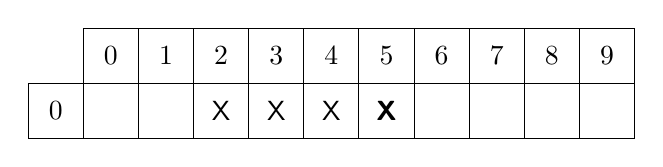
\begin{tikzpicture}[scale=0.7]
\draw (0,1)--(10,1);
\draw (-1,0)--(10,0);
\draw (-1,-1)--(10,-1);
\foreach \x in {0,1,...,10}{
\draw (\x,1)--(\x,-1);
}
\draw (-1,0)--(-1,-1);
\foreach \x in {0,1,...,9}{
\draw (\x+0.5,0.5) node{\x};
}
\draw (-0.5, -0.5) node{$0$};
\draw (5.5, -0.5) node{\textbf{\textsf{X}}};

\draw (2.5, -0.5) node{\textsf{X}};
\draw (3.5, -0.5) node{\textsf{X}};
\draw (4.5, -0.5) node{\textsf{X}};
\end{tikzpicture}\\
\textit{La case $(4,0)$ est augmentée de 1
}\end{center}

\item Le bateau est à cheval sur la case $(5,0)$ (2 possibilités) :
\begin{center}

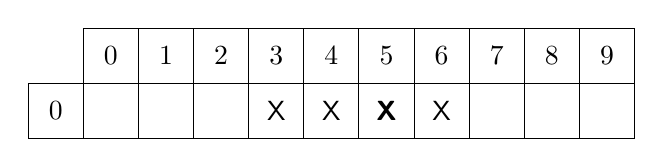
\begin{tikzpicture}[scale=0.7]
\draw (0,1)--(10,1);
\draw (-1,0)--(10,0);
\draw (-1,-1)--(10,-1);
\foreach \x in {0,1,...,10}{
\draw (\x,1)--(\x,-1);
}
\draw (-1,0)--(-1,-1);
\foreach \x in {0,1,...,9}{
\draw (\x+0.5,0.5) node{\x};
}
\draw (-0.5, -0.5) node{$0$};
\draw (5.5, -0.5) node{\textbf{\textsf{X}}};

\draw (6.5, -0.5) node{\textsf{X}};
\draw (3.5, -0.5) node{\textsf{X}};
\draw (4.5, -0.5) node{\textsf{X}};
\end{tikzpicture}
%\textit{Les cases $(4,0)$ et $(6,0)$ sont augmentées de 1
%}\end{center}
%
%\begin{center}

\medskip

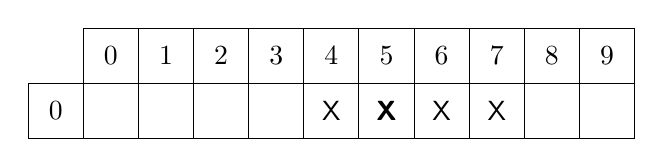
\begin{tikzpicture}[scale=0.7]
\draw (0,1)--(10,1);
\draw (-1,0)--(10,0);
\draw (-1,-1)--(10,-1);
\foreach \x in {0,1,...,10}{
\draw (\x,1)--(\x,-1);
}
\draw (-1,0)--(-1,-1);
\foreach \x in {0,1,...,9}{
\draw (\x+0.5,0.5) node{\x};
}
\draw (-0.5, -0.5) node{$0$};
\draw (5.5, -0.5) node{\textbf{\textsf{X}}};

\draw (6.5, -0.5) node{\textsf{X}};
\draw (7.5, -0.5) node{\textsf{X}};
\draw (4.5, -0.5) node{\textsf{X}};
\end{tikzpicture}\\
\textit{Les cases $(4,0)$ et $(6,0)$ sont augmentées de 2
}\end{center}

\item Le bateau rentre à droite de la case $(5,0)$ :

\begin{center}
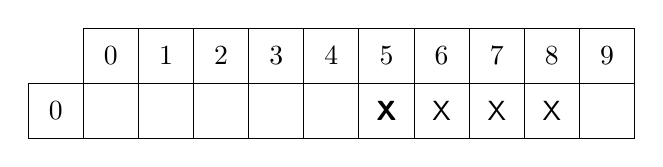
\begin{tikzpicture}[scale=0.7]
\draw (0,1)--(10,1);
\draw (-1,0)--(10,0);
\draw (-1,-1)--(10,-1);
\foreach \x in {0,1,...,10}{
\draw (\x,1)--(\x,-1);
}
\draw (-1,0)--(-1,-1);
\foreach \x in {0,1,...,9}{
\draw (\x+0.5,0.5) node{\x};
}
\draw (-0.5, -0.5) node{$0$};
\draw (5.5, -0.5) node{\textbf{\textsf{X}}};

\draw (6.5, -0.5) node{\textsf{X}};
\draw (7.5, -0.5) node{\textsf{X}};
\draw (8.5, -0.5) node{\textsf{X}};
\end{tikzpicture}\\
\textit{La case $(6,0)$ est augmentée de 1
}\end{center}
\end{enumerate} 
Au final, la case $(4,0)$ admet 3 bateaux horizontaux de taille 4 et idem pour la case $(6,0)$.

Si la case $(3,0)$ avait été jouée et manquée nous aurions obtenu 1 bateau horizontal de taille 4 possible sur la case $(4,0)$ et 2 sur la case $(6,0)$ :

\begin{center}
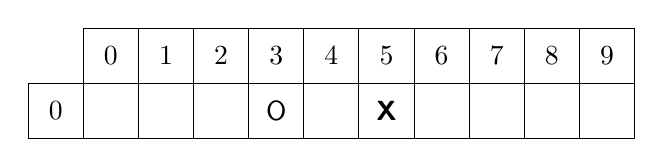
\begin{tikzpicture}[scale=0.7]
\draw (0,1)--(10,1);
\draw (-1,0)--(10,0);
\draw (-1,-1)--(10,-1);
\foreach \x in {0,1,...,10}{
\draw (\x,1)--(\x,-1);
}
\draw (-1,0)--(-1,-1);
\foreach \x in {0,1,...,9}{
\draw (\x+0.5,0.5) node{\x};
}
\draw (-0.5, -0.5) node{$0$};
\draw (5.5, -0.5) node{\textbf{\textsf{X}}};

\draw (3.5, -0.5) node{\textsf{O}};
\end{tikzpicture}\\
\end{center}

Une fois que le compte des bateaux possibles a été effectué sur chacune des cases adjacentes, on crée une liste \texttt{probas\_liste} contenant des tuples de la forme \texttt{(case, probas[case])} que l'on ordonne en ordre décroissant de possibilités grâce à l'instruction \texttt{sorted(probas\_liste, key=lambda proba: proba[1], reverse = True)} et que l'on retourne.

\subsection{Deuxième tir}
Lors du deuxième tir (c'est à dire sur la première case de la file d'attente), on peut soit toucher, soit manquer.
\subsubsection{Deuxième tir touché}
Si on touche alors, grâce à la méthode \texttt{Ordi.update\_queue\_touche(self)}, on détermine la direction du bateau (horizontal ou vertical) en comparant les coordonnées de \texttt{Ordi.case\_courante} et \texttt{Ordi.case\_touchee} et on enlève les cases de la file d'attente qui ne sont pas dans la bonne direction. On ajoute enfin la case à l'extrémité de la configuration créée à la file d'attente et on met à jour la liste \texttt{Ordi.liste\_touches}. L'algorithme de cette partie est donné en annexe \ref{algo_liste}, page \pageref{update_queue_touche}.
\subsubsection{Deuxième tir manqué}
Si on manque, alors on a peut-être bloqué une direction.\\
La méthode \texttt{Ordi.update\_queue\_manque(self)} se charge de cette vérification et élimine la case en face de la case jouée si besoin de la file d'attente.\\
Regardons un exemple. Imaginons que le plus petit bateau à trouver soit de taille 4 et que la première case touchée soit la case $(3,0)$. Nous venons de manquer la case $(4,0)$. Alors le bateau de taille 4 ne rentre plus horizontalement et on peut éliminer la case $(2,0)$ :

\begin{center}
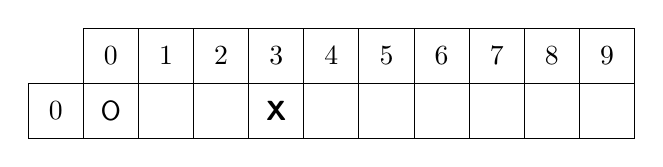
\begin{tikzpicture}[scale=0.7]
\draw (0,1)--(10,1);
\draw (-1,0)--(10,0);
\draw (-1,-1)--(10,-1);
\foreach \x in {0,1,...,10}{
\draw (\x,1)--(\x,-1);
}
\draw (-1,0)--(-1,-1);
\foreach \x in {0,1,...,9}{
\draw (\x+0.5,0.5) node{\x};
}
\draw (-0.5, -0.5) node{$0$};

\draw (3.5, -0.5) node{\textbf{\textsf{X}}};

%\draw (5.5, -0.5) node{\textsf{O}};
\draw (0.5, -0.5) node{\textsf{O}};
\end{tikzpicture}\\
\textit{À ce niveau, le bateau de taille 4 rentre horizontalement.}
\end{center}
%\medskip
\begin{center}
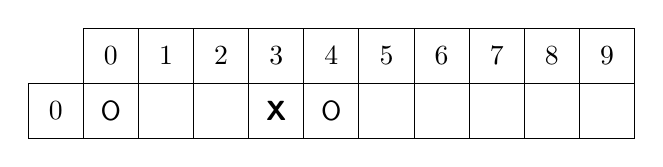
\begin{tikzpicture}[scale=0.7]
\draw (0,1)--(10,1);
\draw (-1,0)--(10,0);
\draw (-1,-1)--(10,-1);
\foreach \x in {0,1,...,10}{
\draw (\x,1)--(\x,-1);
}
\draw (-1,0)--(-1,-1);
\foreach \x in {0,1,...,9}{
\draw (\x+0.5,0.5) node{\x};
}
\draw (-0.5, -0.5) node{$0$};

\draw (3.5, -0.5) node{\textbf{\textsf{X}}};

%\draw (5.5, -0.5) node{\textsf{O}};
\draw (4.5, -0.5) node{\textsf{O}};
\draw (0.5, -0.5) node{\textsf{O}};
\end{tikzpicture}\\
\textit{Après ce coup, le bateau de taille 4 ne rentre plus horizontalement et on peut éliminer la case $(2,0)$.}
\end{center}
Pour ce faire, on détermine la direction dans laquelle on vient de tirer en comparant les coordonnées de \texttt{Ordi.case\_courante} et \texttt{Ordi.case\_touchee} et on regarde si le plus petit bateau rentre dans la direction en face. L'algorithme de cette partie est donné en annexe \ref{algo_liste}, page \pageref{update_queue_manque}.


\subsection{Tirs suivants}
Une fois que la direction du bateau est déterminée, à chaque fois qu'on touche une case, on ajoute à la file d'attente sa case adjacente dans la bonne direction si elle est vide.

Enfin on s'arrête lorsque la file d'attente est vide (on a manqué les deux extrémités) ou lorsque la taille du bateau touché est égale à la plus grande taille du bateau sur la grille avec \texttt{Ordi.test\_plus\_grand(self)} et, dans ce cas, on vide la file d'attente. 
%La méthode \texttt{Ordi.liste\_touches} permet de garder la trace des cases touchées sur ce bateau et d'en déterminer le nombre de cases.

Au prochain tour, on sait qu'un bateau vient d'être coulé lorsque la file d'attente est vide et \texttt{Ordi.liste\_touches} ne l'est pas. Dans ce cas on marque ses cases adjacentes comme impossibles et on l'enlève de la liste des bateaux à chercher. On n'a plus alors qu'à repartir dans une phase de tir en aveugle jusqu'à ce qu'on ait terminé la grille.
%\newpage
%\section{Algorithme complet}
%Voici l'algorithme complet de la résolution :
%
%\begin{algo1}
%La file d'attente est une liste vide\\
%liste\_touches est une liste vide\\
%Tant que le grille n'est pas résolue :\\
%\tab{1}Si la file d'attente est vide :\\
%\tab{2}Si liste\_touches n'est pas vide :\\
%\tab{3}On enlève le bateau de taille len(liste\_touches)\\
%\tab{3}On élimine les cases adjacentes à celles de liste\_touches\\
%\tab{3}On vide liste\_touches\\
%\tab{2}On élimine les zones trop petites\\
%\tab{2}case\_courante reçoit une case en aveugle (suivant le niveau)\\
%\tab{1}Sinon :\\
%\tab{2}case\_courante reçoit le premier élément de la file d'attente\\
%\tab{2}On enlève cette case de la file d'attente\\
%\tab{1}On tire sur case\_courante\\
%\tab{1}Si on a touché :\\
%\tab{2}Si liste\_touches est vide :\\
%\tab{3}On ajoute case\_courante dans liste\_touches\\
%\tab{3}case\_courante\sto case\_touchee\\
%\tab{3}On ajoute ses cases adjacentes dans la file d'attente\\
%\tab{4}(en testant également les directions impossibles éventuelles)\\
%\tab{2}Sinon :\\
%\tab{3}Si len(liste\_touches) == 1 :\\
%\tab{4}On détecte la direction du bateau\\
%\tab{3}On met à jour la file d'attente\\
%\tab{4}(avec la case adjacente à case\_courante dans la bonne direction)\\
%\tab{2}Si le bateau touché est le plus grand restant :\\
%\tab{3}On vide la file d'attente\\
%\tab{1}Sinon :\\
%\tab{2}Si len(liste\_touches) == 1 :\\
%\tab{3}On met à jour la file d'attente\\
%\tab{4}(on élimine éventuellement la case en face de case\_touchee)\\
%On affiche le nombre de coups\\
%\end{algo1}


%-------------------------------------------------------------
\begin{comment}
\newpage

\section{Étude statistique}
Le module \texttt{bn\_stats.py} fournit, dans la classe \texttt{Stats}, les outils pour analyser statistiquement une distribution de valeurs (calculs des indicateurs statistiques classiques, représentation en histogramme et diagramme en boîte grâce aux modules \texttt{numpy} et \texttt{matplotlib}).

Cette classe fournit également les outils pour sauvegarder et charger la liste des résultats bruts dans un fichier texte pour des analyses plus poussées futures.

Un test de l'algorithme de résolution sur $n=1\,000\,000$ parties donne les résultats suivants :

\begin{center}\label{histo_algo}
\fbox{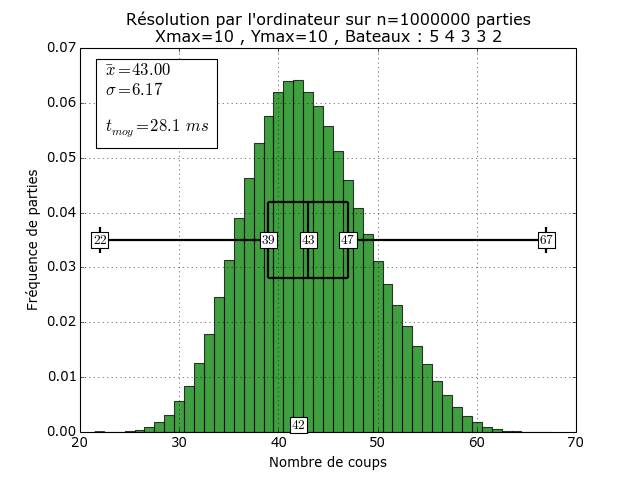
\includegraphics[scale=0.7]{./media/distrib_1000000.png}}
\end{center}

Notons les excellentes performances avec une moyenne de 42,06 coups pour un temps de résolution moyen de seulement 31,2 ms\footnote{Temps mesuré sur un processeur Intel Core i7 4800-MQ à 2,7 Ghz} par partie.

La liste des données obtenues est donnée en annexe \ref{annexe_stats} page \pageref{annexe_stats}.

%La forme de cette distribution semble correspondre à une loi normale asymétrique. Ce résultat sera développé en annexe \ref{annexe_stats} page \pageref{annexe_stats}.

\end{comment}
